%%
%% LinkedListLab (c) 2021-24 Christopher A. Bohn
%%
%% Assignment writeup licensed under the Creative Commons Attribution 4.0 International License
%% https://creativecommons.org/licenses/by/4.0/
%%

\documentclass[12pt]{article}
\usepackage{booktabs}

%%
%% labs/common/assignment.tex
%% (c) 2021-23 Christopher A. Bohn
%%
%% Licensed under the Apache License, Version 2.0 (the "License");
%% you may not use this file except in compliance with the License.
%% You may obtain a copy of the License at
%%     http://www.apache.org/licenses/LICENSE-2.0
%% Unless required by applicable law or agreed to in writing, software
%% distributed under the License is distributed on an "AS IS" BASIS,
%% WITHOUT WARRANTIES OR CONDITIONS OF ANY KIND, either express or implied.
%% See the License for the specific language governing permissions and
%% limitations under the License.
%%

\usepackage{addfont}
\usepackage{amsmath}
\usepackage{amssymb}
\usepackage{animate}
\usepackage{bold-extra}
\usepackage{cancel}
\usepackage{caption}
\usepackage{ccicons}
\usepackage{enumitem}
\usepackage{etoolbox}
\usepackage{fancyhdr}
\usepackage{fullpage}
\usepackage{graphicx}
\usepackage{hyperref}
\usepackage[utf8]{inputenc}
\usepackage[procnames]{listings}
%\usepackage{media9}
\usepackage{multicol}
\usepackage{subfig}
\usepackage{textcomp}
\usepackage{tikz}
\usepackage[americanresistor]{circuitikz}
%\usepackage{tikz-uml}
\usetikzlibrary{automata,positioning,arrows}
\usepackage[normalem]{ulem}
\usepackage{wrapfig}
\usepackage{xcolor}
%\usepackage[dvipsnames]{xcolor}
\definecolor{LightGreen}{rgb}{0.88,1,0.88}

\lstset{language=C, tabsize=4, upquote=true, basicstyle=\ttfamily}
\newcommand{\function}[1]{\textbf{\lstinline{#1}}}
\setlength{\headsep}{0.7cm}
\hypersetup{colorlinks=true}

%% CREDIT FOR MARKERLESSFOOTNOTE WHERE CREDIT IS DUE: https://tex.stackexchange.com/questions/30720/footnote-without-a-marker?answertab=scoredesc#tab-top
\newcommand\markerlessfootnote[1]{%
    \begingroup
    \renewcommand\thefootnote{}\footnote{#1}%
    \addtocounter{footnote}{-1}%
    \endgroup
}

\newcommand{\pagelayout}{
    \pagestyle{fancy}
    \fancyhf{}
    \lhead{\coursenumber}
    \chead{\ Lab \labnumber: \labname}
    \rhead{\courseterm}
    \cfoot{\shortlabname-\thepage}
}

\newcommand{\labidentifier}{
    \title{\ Lab \labnumber}
    \author{\labname}
    \date{Due: \duedate}
    \maketitle

    \textit{\collaborationrules}
    \markerlessfootnote{\tiny{\ifdefstring{\instructorname}{Christopher A. Bohn}{Assignment}{Original assignment} and starter code \copyright\ Christopher A. Bohn, licensed under the Creative Commons Attribution 4.0 International License~\ccby\ and under the Apache License Version 2.0, respectively.}}
    \ifdefstring{\instructorname}{Christopher A. Bohn}{}{\markerlessfootnote{\tiny{Configured for \coursenumber\ at \institutename\ by \instructorname.}}}

    \begin{description}
        \item[Obtaining the starter code] \filesource
        \item[Runtime environment] We will grade this assignment by compiling and running it on \runtimeenvironment;
            you should compile and test your code on \runtimeenvironment\ before turning it in.
        \item[Submitting your work] \filesubmission
    \end{description}
}

% display module fonts for hardware kit
% use with the Capital baseball "matrix printer" font collection (https://www.ctan.org/tex-archive/fonts/capbas/)
% Identifying the specific font in the assignment sheet is deprecated
%   -- instead, set the `usedisplayfont` boolean and the `displaymodule` variable in semester.tex,
%      and \display{...} in the assignment sheet

\addfont{OT1}{d7seg}{\dviiseg}
\addfont{OT1}{deseg}{\deseg}
\addfont{OT1}{necker}{\necker}

\providebool{usedisplayfont}

\newcommand{\display}[1]{
    \ifboolexpe{bool{usedisplayfont}}{
        \ifdefstring{\displaymodule}{MAX7219digits}{{\dviiseg #1}}{}
        \ifdefstring{\displaymodule}{MAX7219matrix}{{\deseg #1}}{}
        \ifdefstring{\displaymodule}{LCD1602}{{\necker #1}}{}
        % We don't yet have a Cow Pi configuration with 14-segment displays, so no \deseg yet
    }{
        \texttt{#1}
    }
}

\newcommand{\rubricitem}[2]{\item[\underline{\hspace{1cm}} +#1] #2}
\newcommand{\bonusitem}[2]{\item[\underline{\hspace{1cm}} Bonus +#1] #2}
\newcommand{\penaltyitem}[2]{\item[\underline{\hspace{1cm}} -#1] #2}
\newcommand{\checkoffitem}[1]{\item (\phantom{xxx}) #1}
\newcommand{\precheckoffitem}[1]{\item [] (\phantom{xxx}) #1}

\newcommand{\institutename}{University of Nebraska-Lincoln}
\newcommand{\instructorname}{Christopher A. Bohn}
\newcommand{\coursenumber}{CSCE~231}
\newcommand{\cstwo}{CSCE~156, RAIK~184H, or SOFT~161}
\newcommand{\courseterm}{Spring 2025}
\newcommand{\labnumber}{10}
\newcommand{\labname}{Using Polling with Memory-Mapped Input/Output}
\newcommand{\shortlabname}{PollingLab}
\newcommand{\duedate}{Week of April 14, before the start of your lab section}
\newcommand{\pathone}{chap09/io/memory-mapped}
\newcommand{\pathtwo}{chap09/system-descriptions/number-builder}
\newcommand{\filesource}{Download \startercode\ from Canvas, or copy \startercode\ from {\footnotesize$\sim$}cbohn2/csce231 on \textit{nuros.unl.edu}}
\newcommand{\filesubmission}{When you have completed this assignment, submit \requiredfiles\ to the assignment in Canvas.}
\newcommand{\runtimeenvironment}{a Cow Pi development board with a \processor\ microcontroller}
\newcommand{\startercode}{pollinglab.zip or pollinglab.tar}
\newcommand{\requiredfiles}{\textit{io\_functions.c} and \textit{number\_builder.c}}
\newcommand{\buildsystem}{platformio}
\newcommand{\processor}{RP2040}
\newcommand{\lowercaseprocessor}{rp2040}
\newcommand{\collaborationrules}{During your scheduled lab time, you may, \textbf{but are not required to}, form a partner group of 2 students.
    When necessary, there may be a group of 3 students.
    During your scheduled lab time, and until the end of your lab day, you may discuss problem decomposition and solution design with your lab partner.
    After your scheduled lab day, you may discuss concepts and syntax with other students, but you may discuss solutions only with the professor and the TAs.
    Sharing code with or copying code from another student or the internet is prohibited.
}
\newcommand{\policyforcodethatdoesnotcompile}{\subsection*{No Credit for Uncompilable Code}
    If the TA cannot create an executable from your code, then your code will be assumed to have no functionality.\footnote{
        At the TA's discretion, if they can make your code compile with \textit{one} edit (such as introducing a missing semicolon) then they may do so and then assess a 10\% penalty on the resulting score.
        The TA is under no obligation to do so, and you should not rely on the TA's willingness to edit your code for grading.
        If there are multiple options for a single edit that would make your code compile, there is no guarantee that the TA will select the option that would maximize your score.
    }
    Before turning in your code, be sure to compile and test your code on \runtimeenvironment\ with the original driver code, the original header file(s), and the original \textit{Makefile}.}
\newcommand{\latepolicy}{\subsection*{Late Submissions}
    This assignment is due before the start of your lab section.
     After you have exhausted your grace days, we will accept late turn-ins up to one hour late, assessing a 10\% penalty on these late submissions.
    After you have exhausted your grace days, any work turned in more than one hour late will not be graded.}
\newcommand{\softwareengineeringfrontmatter}{\section*{No Spaghetti Code Allowed}
        In the interest of keeping your code readable, you may \textit{not} use
        any \lstinline{goto} statements, nor may you use any
        \lstinline{continue} statements, nor may you use any \lstinline{break}
        statements to exit from a loop, nor may you have any functions
        \lstinline{return} from within a loop.}
\newcommand{\softwareengineeringpenalties}{\penaltyitem{1}{for each \lstinline{goto} statement,
            \lstinline{continue} statement, \lstinline{break} statement used to
            exit from a loop, or \lstinline{return} statement that occurs within
            a loop.}}
\newcommand{\scenariointroduction}{    Archie walks up to you, along with Herb Bee from Eclectic Electronics.
    Herb is holding a tangled mess of electronics.
    Archie explains, ``Herb here has developed a prototype of a device that he thinks will be useful for our physical security needs, as well as a few other applications around here. He calls it the \textit{Cow Pi}.''

    You look at the device in Herb's hands and see the Raspberry Pi Pico central to the circuit.
    ``I suppose the `\textit{-Pi}' suffix is because it uses a Raspberry Pi Pico?''
+        
    Herb replies, ``Um, yeah, sure.
 We considered using an Arduino Nano, but \textit{Cowduino} isn't very punny, is it?''

    Archie chimes in, ``Maybe with the right emphasis: \textit{Cow-DOO-ino}.''

    ``That's kind of subtle, don't you think? How will people know to put the emPHAsis on that sylLAble?''
    
    ``I think we're getting off topic here,'' you point out.
    ``How can I help?''

    ``Oh, right,'' Herb says, ``We'd like you to kick its proverbial tires.
    Let's start off with something simple, like a number builder tool.''}
\newcommand{\scenariowrapup}{Herb looks over your work.
    ``Hmm, yes. I think this is coming along nicely.
    Let's run a few more tests.''

    Archie storms into the room.
    ``We have \textit{got} to do something about security!
    How's that doodad coming along? 
    Because there's now a half-man/half-fly in the labs going on-and-on about Chaos Theory and how if we just give him a MacBook and a spaceship then he'll be able to get the Lord of Thunder to travel across the 8th Dimension.
    Is that thing just about ready?''

    Herb shakes his head, ``No, not quite yet. It should be ready in about a week.''}

../../PointerLab/assignment/linked-list-nodes.tex

\lstset{language=c, numbers=left, showstringspaces=false,
    moredelim = [s][\ttfamily]{/*}{*/} % I shouldn't need this parameter!
}
%%
%%
% Credit where credit is due. Skipping line numbers from
% https://tex.stackexchange.com/questions/476100/lstlisting-line-number-gaps
\makeatletter
\let\orig@lstnumber=\thelstnumber

\newcommand\lstsetnumber[1]{\gdef\thelstnumber{#1}}
\newcommand\lstresetnumber{\global\let\thelstnumber=\orig@lstnumber}
\makeatother
%%
%%


\pagelayout
\begin{document}
    \labidentifier

    \pdfbookmark[1]{Frontmatter}{frontmatter}                       The purpose of this assignment is to give you more confidence in C programming
and to begin your exposure to the underlying bit-level representation of data.

The instructions are written assuming you will edit and run the code on
\runtimeenvironment. If you wish, you may edit and run the code
in a different environment; be sure that your compiler suppresses no warnings,
and that if you are using an IDE that it is configured for C and not C++.

\section*{Learning Objectives}

After successful completion of this assignment, students will be able to:
\begin{itemize}
    \item Use the ASCII table to determine the corresponding integer values of C
    \lstinline{char} values.
    \item Apply arithmetic operators and comparators to C \lstinline{}{char} values.
    \item Construct and use a bitmask.
    \item Use bitwise operators and bit shift operators to create and modify values.
\end{itemize}

\subsection*{Continuing Forward}

Your experience with viewing values as bit patterns will be applicable in
future labs, as will bit masks and bit operations. Some of the functions you
write in this lab will be used in the next lab.

\section*{During Lab Time}

During your lab period, the TAs will demonstrate how to read the ASCII table and
will provide a refresher on bitwise AND, bitwise OR, and left- and right-shifts.
During the remaining time, the TAs will be available to answer questions.

Before leaving lab, \textit{at a minimum} \dots


    \softwareengineeringfrontmatter

    \section*{Scenario}                                             \scenariointroduction

    \section{Assignment Summary}                                    Please familiarize yourself with the entire assignment before beginning.
There are three parts to this assignment.

\subsection{Why are There Letters on Telephone Keypads?}

Once upon a time, telephone exchanges were staffed by operators who would use patch cords on a switchboard to connect callers.
If you needed to make a local-area call to someone whose phone was serviced by a different exchange, then you needed to tell your operator which exchange to connect to.
Letters were assigned to digits so that easy-to-remember -- and audibly-distinctive -- mnemonics could be formed such that the first two letters of the mnemonic that correspond to the 2-digit exchange identifier.
For example, the 86 exchange would use a mnemonic that started with a `T', `U', or `V' and that has as a second letter an `M', `N', or `O' --
so 867--5309 might be ``University 7--5309''.

The presence of letters on telephone dials and (later) telephone keypads allowed for custom phone numbers that used words formed by the available letters.
For example, a bank's phone number might be 472--2265, aka 472--BANK.
Less fictionally, 1--800--FLOWERS was used by a company that partnered with florists to allow people to have bouquets delivered anywhere in the U.S\@.

When the Short Message Service protocol was introduced to allow text-based communication by taking advantage of unused bytes in the handshake between cellular phones and the cell network, naturally the letters that were already present on the keypad were used to tap out messages.

While QWERTY keyboards on smartphones have largely replaced the 10-digit keypad for text entry, the letters remain, waiting for the next clever use\dots

\subsection{Constraints} \label{subsec:constraints}

You may \textit{not} poll the matrix keypad nor the pushbuttons to determine if they have been pressed.
You must use interrupts to determine if a key or button has been pressed.
Once an interrupt has fired, you may scan the matrix keypad or read the pushbuttons to determine which key has been pressed or whether the button has been pressed or released.

You may use any features that are part of the C standard if they are supported by the compiler.
You may use the constants and functions provided in the starter code.

\subsubsection{Constraints on the Arduino core}

You may \textit{not} use any libraries, functions, macros, types, or constants from the Arduino core.

%\subsubsection{Constraints on AVR-libc}
%
%You may use any AVR-specific functions, macros, types, or constants of avr-libc.\footnote{
%    \url{https://www.nongnu.org/avr-libc/user-manual/index.html}
%}

\ifdefstring{\processor}{ATmega328P}{
    \subsubsection{Constraints on AVR-libc}

    You may not use any AVR-specific functions, macros, types, or constants of avr-libc.\footnote{\url{https://www.nongnu.org/avr-libc/user-manual/index.html}}
}{}
\ifdefstring{\processor}{RP2040}{
% TODO: parameterize this (when we eventually port to the bare-metal Arduino toolchain, and to the Pico SDK)
    \subsubsection{Constraints on MBED OS}

    You may not use any functions, macros, types or constants from MBED that are not part of the C standard.\footnote{\url{https://os.mbed.com/docs/mbed-os/v6.16/introduction/index.html}}
}{}

\subsubsection{Constraints on the CowPi library}

You may use any functions provided by the CowPi\footnote{
    \url{https://cow-pi.readthedocs.io/en/latest/library.html}
}
and the CowPi\_stdio\footnote{
    \url{https://cow-pi.readthedocs.io/en/latest/stdio.html}
} libraries,
and you may use any data structures\footnote{
    \url{https://cow-pi.readthedocs.io/en/latest/microcontroller.html}
} provided by the CowPi library.

\subsubsection{Constraints on other libraries}

You may \textit{not} use any libraries beyond those explicitly identified here.


    \section{Stray Values in Memory} \label{sec:archiesCode}        ../../common/assignment/archies-code.tex

    \section{TL;DR} \label{sec:tldr}                                Sections~\ref{subsec:tldrBusinessRules}--\ref{subsec:tldrInsertionSort} are concise versions of Sections~\ref{subsec:BusinessRules}--\ref{subsec:TestingChallengeResponse};
if you need more-detailed instructions, see the appropriate subsection in Section~\ref{sec:challengeResponse}.
Sections~\ref{subsec:BuildingLinkedList}--\ref{subsec:MergingNodes} already offer concise instructions to implement the linked list;
we shall not unnecessarily duplicate them here.

\subsection{The Books} \label{subsec:tldrBusinessRules}

    The starter code includes six files that you can use as inputs.
    Three are pre-sorted, and three aren't.
    Two are short, only 7 words, which can be useful for debugging.
    Two are moderate-sized, 74-125 words, to give you confidence in the correctness of your solution.
    Two are large, in excess of 74,000 words, which are useful to reveal whether you have any memory leaks in your code.

    Each book file, ``\textit{file}'', has a corresponding ``\textit{file}-table.md'' that contains a Markdown-formatted table of the challenge words, the number of occurrences for each challenge word, and the corresponding response word.
    You may use these files to confirm the correctness of your solution.

%    The challenge-response app has rules to define how to find the appropriate response word.
%    The starter code already implements these rules, but that implementation will only work if your code builds an alphabetically-sorted list of words that occur in a file and the number of occurrences of each word.

    Note that alphabetization is case-insensitive for this application.


\subsection{Word Entries}

    The \lstinline{word_entry_t} type is defined in \textit{word\_entry.h}:

    \lstinputlisting[linerange=28-31, firstnumber=28]{../starter-code/word_entry.h}

    There are a handful of function prototypes in \textit{word\_entry.h} that encapsulate this datatype.

    \subsubsection{Creating and Destroying Word Entries}

        The \function{create_word_entry()} function allocates space for a \lstinline{word_entry_t}, and the \function{delete_word_entry()} function releases that memory.
        The \function{create_word_entry()} function, however, does not yet initialize the word entry.

        \begin{description}
            \checkoffitem{In \function{create_word_entry()}'s \lstinline{else} block, copy \lstinline{word} into \lstinline{word_entry}'s \lstinline{word} field.}
            \checkoffitem{In \function{create_word_entry()}'s \lstinline{else} block, set \lstinline{word_entry}'s \lstinline{occurrences} field to 0.}
        \end{description}

        You do not need to make any changes to \function{delete_word_entry()}.

    \subsubsection{Accessors and Mutators \\ \footnotesize{\textit{aka}, Getters and Setters}}

        \begin{description}
            \checkoffitem{In \function{increment_count()}, increase the word entry's number of occurrences by one.}
            \checkoffitem{In \function{get_count()}, return the number of occurrences.}
            \checkoffitem{In \function{get_word()}, return a pointer to the word entry's word. (Do \textit{not} make a copy of the word.)}
        \end{description}

    \paragraph{Testing Your Changes}

        You can build an executable that uses H.Awk's array-backed list with the command \\
        \verb+make arraylist+ \\
        or, if you want to limit each \function{malloc()} call to no more than 256 bytes, then use the command \\
        \verb+make arraylist OPTION="-DHOBBLE"+

        \begin{description}
            \checkoffitem{Build and run the executable.}
            \checkoffitem{Select task 1, ``Test word\_entry''.}
            \checkoffitem{Select function 1, ``create\_word\_entry()'', and enter a word when prompted.}
            \checkoffitem{Use fuctions 3 (``increment\_count()''), 4 (``get\_count()''), and 5 (``get\_word()'') to test your code.}
            \checkoffitem{Continue to test until you discover a bug or are satisfied that your implementations are correct.}
            \checkoffitem{When you have finished, use function 2 (``delete\_word\_entry()'') to release the word entry's memory, then select 0 to return to the main menu, and then select 0 to exit the program.}
            \begin{itemize}
                \item Note: whenever you return to the main menu, any existing list will be deleted.
                No memory references survive when moving between one main-menu-option and another.
            \end{itemize}
        \end{description}


\subsection{Alphabetical Functions}

    \subsubsection{Making a Lowercase Copy of a Word}

        \begin{description}
            \checkoffitem{Implement the \function{word_to_lowercase()} function.}
        \end{description}

    \subsubsection{Comparing Words}

        \begin{description}
            \checkoffitem{Implement the \function{words_are_equal()} function.}
            \checkoffitem{Implement the \function{word1_is_earlier_than_word2()} function.}
            \checkoffitem{Implement the \function{word1_is_later_than_word2()} function.}
        \end{description}

    \paragraph{Testing Your Changes}

        \begin{description}
            \checkoffitem{Build and run the executable.}
            \checkoffitem{Select task 3, ``Test alphabetical functions'', and enter words when prompted.}
            \checkoffitem{Continue to test until you discover a bug or are satisfied that your implementations are correct.}
            \checkoffitem{When you have finished, select 0 to exit the program.}
        \end{description}


\subsection{Preparing to Work with Lists}

    Like \lstinline{word_entry_t}, the \lstinline{list_t} and the \lstinline{iterator_t} datatypes have functions to encapsulate them.
    In the case of \lstinline{list_t} and \lstinline{iterator_t}, however, this encapsulation is essential because the code in \textit{sorted\_word\_entries.c} has access to the type declaration but not the type definition.

    \begin{description}
        \checkoffitem{Review the datatypes and functions declared in \textit{list.h}.}
    \end{description}

    A list is abstractly modeled as having a sequence of word entries and an iterator that points to the ``current'' word entry.
    The iterator can point to anywhere between the first word entry and the last word entry.

    \begin{description}
        \checkoffitem{Review the \function{test_list()} function in \textit{list-test.c} to see uses of the \lstinline{list_t} and \lstinline{iterator_t} functions.}
        \checkoffitem{Run the arraylist executable, selecting task 2 (``Test list'') to observe the behavior of the \lstinline{list_t} and \lstinline{iterator_t} functions.}
    \end{description}


\subsection{Inserting Words}

    \subsubsection{Limited Implementation}

        You will receive half of the credit for \function{insert_word()} if it works on pre-sorted books.
        If you choose to use this implementation:
        \begin{description}
            \checkoffitem{Implement \function{insert_word()} for pre-sorted books}
            \checkoffitem{Test this implementation and move on to implementing a linked list}
            \checkoffitem{Return to this sub-problem later to attempt a more-general implementation}
        \end{description}

    \subsubsection{Insertion Sort} \label{subsec:tldrInsertionSort}

        To receive full credit for \function{insert_word()}, it must work on books that are not pre-sorted.
        If you choose to use this implementation:
        \begin{description}
            \checkoffitem{Implement \function{insert_word()} such that:}
            \begin{itemize}
                \item The word is placed at the end of the list
                \item If the word is not in its proper location, then it is moved to is proper location
                \item Once in its proper location, if there is another word entry with the same word, then the two word entries are combined
            \end{itemize}
        \end{description}

    \paragraph{Testing Your Changes}

        \begin{description}
            \checkoffitem{Build and run the executable.}
            \checkoffitem{Use tasks 4--6 to test \function{insert_word()} until you discover a bug or are satisfied that your implementation is correct.}
            \checkoffitem{Use task 7 to test your code with the files of words.}
            \checkoffitem{When you have finished, select 0 to exit the program.}
        \end{description}


\subsection{Implementing a Linked List}

    Sections~\ref{subsec:BuildingLinkedList}--\ref{subsec:MergingNodes} are already fairly concise;
    we shall not duplicate them here.




    \section{Challenge and Response} \label{sec:challengeResponse}  \subsection{Business Rules} \label{subsec:BusinessRules}

% TODO: Parameterize business rules

\begin{itemize}
    \item All of the book's words are sorted alphabetically without regard to capitalization (for example, ``hello'' occurs after ``Hear'' and before ``HELP'')
    \item The word occurs \textit{occurrences} times in the book
%    \item If $occurrences$ is an even number then the response word is the word is $occurrences$ places \textbf{after} the challenge word in the alphabetized list;
%    if the challenge word is less than $occurrences$ places from the start of the list then the response word is the first word in the list
%    \item If $occurrences$ is an odd number then the response word is the word $occurrences$ places \textbf{before} the challenge word in the alphabetized list;
%    if the challenge word is less than $occurrences$ places from the end of the list then the response word is the last word in the list
\end{itemize}

As a simple example, look at the \textit{Food} file.
After sorting and counting, we have:

\begin{center}
    \begin{tabular}{cc}
        \textit{word} & \textit{occurrences} \\ \hline
        apple       & 7 \\
        banana      & 4 \\
        carrot      & 15 \\
        date        & 3 \\
        eggplant    & 2 \\
        fig         & 6 \\
        granola     & 9 \\
        horseradish & 9 \\
        ice         & 6 \\
        jelly       & 3 \\
        kale        & 1 \\
        lemon       & 2 \\
        mango       & 8 \\
        naan        & 7 \\
        orange      & 5 \\
        pineapple   & 1 \\
        quinoa      & 11 \\
        raisin      & 4 \\
        spaghetti   & 10 \\
        tomato      & 12 \\
    \end{tabular}
\end{center}

You break the problem down into three sub-problems:

\begin{enumerate}
    \item Designing the Data Structure and Its Algorithms
    \item Alphabetizing Words
    \item Inserting Words
%    \item Responding to a Challenge
\end{enumerate}

\subsubsection*{The Books}

Four small ``books'' are included with the starter code:

\begin{itemize}
    \item ``Animals'' (sorted, 7 words)
    \item ``Plants'' (unsorted, 7 words)
    \item ``Cars'' (sorted, 74 words)
    \item ``Food'' (unsorted, 125 words)
\end{itemize}

Two real books have also been reduced to one word per line:\footnote{The text for these books was obtained from \href{https://www.gutenberg.org/}{Project Gutenberg}.
In accordance with Paragraph~1.C of the \href{https://www.gutenberg.org/policy/license}{Project Gutenberg License}, all references to Project Gutenberg have been removed from the ``derived works'' that we are distributing.
    (Removing the references to Project Gutenberg was also necessary to ensure that \textit{only} the words from the books are included in the list.)}

\begin{itemize}
    \item Mary Shelly's \textit{Frankenstein; Or, The Modern Prometheus} (filename ``Frankenstein'') \url{https://www.gutenberg.org/ebooks/84} (sorted, 74,363 words)
    \item Arthur Conan Doyle's \textit{The Lost World} (filename ``TheLostWorld'')
    \url{https://www.gutenberg.org/ebooks/139} (unsorted, 77,268 words)
\end{itemize}

The very small files of 7 words can be useful for debugging, and the moderate-sized files of 74--125 words should give you confidence in the correctness of your solution.
The real books of more than 74,000 words will be useful to reveal whether you have any memory leaks in your code.
The files marked as \textit{sorted} have all of their words already in alphabetically sorted order, ignoring capitalization;
the files marked as \textit{unsorted} do not have their words sorted (the words in ``Plants'' and ``Food'' are in a randomly-selected order;
the words in ``TheLostWorld'' appear in the order that they appear in the original \textit{The Lost World}).

Each book file, ``\textit{file}'', has a corresponding ``\textit{file}-table.md'' that contains a Markdown-formatted table of the words and the number of occurrences for each word.
You may use these files to confirm the correctness of your solution.

Throughout the assignment, we note that if building the list takes more than a few seconds, there is a bug in your code;
You should be able to build a list for \textit{Frankenstein} or \textit{The Lost World} in under a second.
Your code may take longer, but it should not take much longer.

\colorbox{yellow}{Some of the tests in \textit{sorted-test.c} will timeout after ten seconds to stop runaway code.} \\
\colorbox{yellow}{To disable this timeout (such as when debugging with breakpoints), compile the code with} \\
\colorbox{yellow}{\texttt{touch sorted-list.c; make OPTION="-DNOTIMEOUT"}} \\
(to re-enable the timeout, use \texttt{touch sorted-test.c; make})

You will earn most of the credit for this lab if your code works for pre-sorted files of up to 200 words.
The remaining credit is for making your code work with unsorted files and, when using files of up to 80,000 words, your code can generate a list and find a word in fewer than 20 seconds.

\vspace{1cm}

H.Awk provides you with the code he worked on.
It turns out that while he finished implemented the array-backed list, he didn't finish the sorting algorithm.
You decide to warm up by finishing the app and then circling back to the linked list.

\subsection{Word Entries}

The \lstinline{word_entry_t} type is defined in \textit{word\_entry.h}:

\lstinputlisting[linerange=28-31, firstnumber=28]{../starter-code/word_entry.h}

You see that there are also a handful of function prototypes in \textit{word\_entry.h} that would nicely encapsulate this datatype.

\subsubsection{Creating and Destroying Word Entries}

The \function{create_word_entry()} function allocates space for a \lstinline{word_entry_t}, and the \function{delete_word_entry()} function releases that memory.
The \function{create_word_entry()} function, however, does not yet initialize the word entry.

\begin{description}
    \checkoffitem{In \function{create_word_entry()}'s \lstinline{else} block, copy \lstinline{word} into \lstinline{word_entry}'s \lstinline{word} field.}
    \checkoffitem{In \function{create_word_entry()}'s \lstinline{else} block, set \lstinline{word_entry}'s \lstinline{occurrences} field to 0.}
\end{description}

When you copy the word, you must actually copy the word and not merely copy the pointer, for two reasons.
The first reason, from a program design perspective, is that you don't know whether the caller might later put a different word in the array that the \lstinline{word} parameter is in, or the caller might even deallocate that array's memory.
The second reason, from a memory perspective, is that an array embedded in a \lstinline{struct} (such as \lstinline{word_entry_t}'s \lstinline{word} field) is effectively a constant pointer and cannot be re-assigned.

You do not need to make any changes to \function{delete_word_entry()}.

\subsubsection{Accessors and Mutators \\ \footnotesize{\textit{aka}, Getters and Setters}}

We want to control the possible changes that other code might make to a word entry.
Indeed, the only reasonable change would be to increase the number of times that the word is found in a book, whenever we encounter that word again.
Similarly, we want to make sure that data that our ``getter'' functions cannot be used by the caller to make changes to the structure's data.
The \function{get_count()} function returns a value, so there's no hazard there.
The \function{get_word()} function returns a pointer to a constant -- while it \textit{is} possible to discard a \lstinline{const} qualifier, doing so will result in a warning that it will result in undefined behavior.
(The array that the pointer points to isn't actually constant, but the caller is obligated to act as though it is.)

\begin{description}
    \checkoffitem{In \function{increment_count()}, increase the word entry's number of occurrences by one.}
    \checkoffitem{In \function{get_count()}, return the number of occurrences.}
    \checkoffitem{In \function{get_word()}, return a pointer to the word entry's word. (Do \textit{not} make a copy of the word.)}
\end{description}

When returning the word entry's word, simply returning the pointer is sufficient -- and desirable.
It is sufficient because the caller is obligated to treat it as a constant.
The alternative, making a copy, is not desirable because the function doesn't expect the caller to provide a destination, which means that the function would have to allocate memory for the destination;
the caller would be unable to later free this memory without discarding the \lstinline{const} qualifier.

\paragraph{Testing Your Changes}

You can build an executable that uses H.Awk's array-backed list with the command \\
\verb+make arraylist+ \\
or, if you want to limit each \function{malloc()} call to no more than 32KB, then use the command \\
\verb+make arraylist "OPTION=-DHOBBLE"+

\begin{description}
    \checkoffitem{Build and run the executable.         \\
        \texttt{0) Quit                                 \\
                1) Test word\_entry                     \\
                2) Test list                            \\
                3) Test alphabetical functions          \\
                4) Test insert\_word (empty list)       \\
                5) Test insert\_word (singleton list)   \\
                6) Test insert\_word (populated list)   \\
                7) Create and print book list           \\
                Select the task you wish to check:}}
    \checkoffitem{Select task 1, ``Test word\_entry''.  \\
        \texttt{0) Return to main menu                  \\
                1) create\_word\_entry()                \\
                2) delete\_word\_entry()                \\
                3) increment\_count()                   \\
                4) get\_count()                         \\
                5) get\_word()                          \\
                Select the function you wish to check:}}
    \checkoffitem{Select function 1, ``create\_word\_entry()'', and enter a word when prompted.}
\end{description}

The word entry will be displayed.
For example, if your word was ``foo'' then the output will be: \\
\texttt{Created --           0 : foo}

\begin{description}
    \checkoffitem{Use fuctions 3 (``increment\_count()''), 4 (``get\_count()''), and 5 (``get\_word()'') to test your code.}
    \checkoffitem{Continue to test until you discover a bug or are satisfied that your implementations are correct.}
    \checkoffitem{When you have finished, use function 2 (``delete\_word\_entry()'') to release the word entry's memory, then select 0 to return to the main menu, and then select 0 to exit the program.}
    \begin{itemize}
        \item Note: whenever you return to the main menu, any existing list will be deleted.
            No memory references survive when moving between one main-menu-option and another.
    \end{itemize}
\end{description}



\subsection{Alphabetical Functions}

\subsubsection{Making a Lowercase Copy of a Word}

Because the book's words should be insensitive to capitalization, we will store the words with all of their letters in lowercase.
In \textit{challenge-response.c}, there is a \function{word_to_lowercase()} function to do just that.

\begin{description}
    \checkoffitem{Implement the \function{word_to_lowercase()} function.}
\end{description}

Unlike keyboardlab, you can use the \function{tolower()} function\footnote{\url{https://en.cppreference.com/w/c/string/byte/tolower}} from \texttt{ctype.h}.

\subsubsection{Comparing Words}

Because the book's words need to be sorted, we need to be able to compare words.
In \textit{challenge-response.c}, there are three functions to do that:
\begin{description}
    \item[words\_are\_equal()] which returns \lstinline{true} if and only if the two words are indistinguishable
    \item[word1\_is\_earlier\_than\_word2()] which returns \lstinline{true} if and only if the first word precedes the second word in an alphabetically-sorted list
    \item[word1\_is\_later\_than\_word2()] which returns \lstinline{true} if and only if the first word follows the second word in an alphabetically-sorted list
\end{description}

\begin{description}
    \checkoffitem{Implement the \function{words_are_equal()} function.}
    \checkoffitem{Implement the \function{word1_is_earlier_than_word2()} function.}
    \checkoffitem{Implement the \function{word1_is_later_than_word2()} function.}
\end{description}

We recommend that you use the \function{strncmp()} function\footnote{\url{https://en.cppreference.com/w/c/string/byte/strncmp}} from \texttt{string.h}.

\paragraph{Testing Your Changes}

You can build an executable that uses H.Awk's array-backed list with the command \\
\verb+make arraylist+ \\
or, if you want to limit each \function{malloc()} call to no more than 32KB, then use the command \\
\verb+make arraylist "OPTION=-DHOBBLE"+

\begin{description}
    \checkoffitem{Build and run the executable.         \\
        \texttt{0) Quit                                 \\
                1) Test word\_entry                     \\
                2) Test list                            \\
                3) Test alphabetical functions          \\
                4) Test insert\_word (empty list)       \\
                5) Test insert\_word (singleton list)   \\
                6) Test insert\_word (populated list)   \\
                7) Create and print book list           \\
                Select the task you wish to check:}}
    \checkoffitem{Select task 3, ``Test alphabetical functions'', and enter words when prompted.}
\end{description}

Each word will be displayed in its lowercase form, and the results of the three comparison functions will be shown.

\begin{description}
    \checkoffitem{Continue to test until you discover a bug or are satisfied that your implementations are correct.}
    \checkoffitem{When you have finished, select 0 to exit the program.}
\end{description}


\subsection{Preparing to Work with Lists}

It is entirely probable that H.Awk, left to his own devices, would simply have used an array instead of making the effort to create an array-backed list with a well-defined abstract model.
Fortunately, someone pulled his strings, and you have available to you an abstract model of a list that can be realized by any number of implementations.

Like \lstinline{word_entry_t}, the \lstinline{list_t} and the \lstinline{iterator_t} datatypes have functions to encapsulate them.
In the case of \lstinline{list_t} and \lstinline{iterator_t}, however, this encapsulation is essential because the code in \textit{sorted\_word\_entries.c} has access to the type declaration but not the type definition.

\begin{description}
    \checkoffitem{Review the datatypes and functions declared in \textit{list.h}.}
\end{description}

A list is abstractly modeled as having a sequence of word entries and an iterator that points to the ``current'' word entry.
The iterator can point to anywhere between the first word entry and the last word entry.

\textcolor{red}{
A good rule of thumb is that if the previous operation returned the iterator, then the iterator is valid;
if the previous operation returned the list, then the iterator is invalid and should not be used.
Attempting to access non-existent word entries beyond the bounds of the list will also invalidate the iterator.
}

\begin{itemize}
    \item The \function{get_iterator()} function sets the iterator to the first word entry, and the \function{iterate_next()} and \function{iterate_previous()} functions cause the iterator to advance and retreat
    \item The \function{has_next()} and \function{has_previous()} functions report whether there are additional word entries in the indicated direction
    \item The \function{get_word_entry()} function retrieves the word entry that the iterator points to, and the \function{get_next_word_entry()} and \function{get_previous_word_entry()} functions retrieve the word entry in the indicated direction
    \item The \function{prepend()} and \function{append()} functions place a word entry at the beginning or end of the list, respectively, setting the iterator to the new word entry
    \item The \function{insert()} function places a new word entry at the iterator's location, and the function{delete()} function removes the word entry at the iterator's location -- both of these functions invalidate the iterator
    \item The \function{swap_next()} and \function{swap_previous()} functions can be used to move a word entry forward and backward
    \item The \function{merge_next()} and \function{merge_previous()} functions can be used to combine a word entry with its neighbor
\end{itemize}

\begin{description}
    \checkoffitem{Review the \function{test_list()} function in \textit{list-test.c} to see uses of the \lstinline{list_t} and \lstinline{iterator_t} functions.}
    \checkoffitem{Run the arraylist executable, selecting task 2 (``Test list'') to observe the behavior of the \lstinline{list_t} and \lstinline{iterator_t} functions.}
\end{description}


\subsection{Inserting Words}

The \function{build_list()} function in \textit{sorted\_word\_entries.c} reads words from a ``book'' and sends them to \function{insert_word()}.
You do not need to implement \function{build_list()}.

The \function{insert_word()} function in \textit{sorted\_word\_entries.c} finds the correct place in the list for a lowercase copy of the word.
If the word is already in the list, then it increments the word's count;
otherwise, it inserts the word into the list.
You will implement \function{insert_word()}.

\subsubsection{Limited Implementation}

The simplest implementation of \function{insert_word()} is to assume that the words in the book are already sorted -- as they are for ``Animals'', ``Cars'', and ``Frankenstein''.
In this case, you know that if the word is already in the list then it is the last word in the list,
and if the word is not already in the list then it belongs at the end of the list.

You will receive half of the credit for \function{insert_word()} if it works on pre-sorted books.
If you choose to use this implementation:
\begin{description}
    \checkoffitem{Implement \function{insert_word()} for pre-sorted books}
    \checkoffitem{Test this implementation and move on to implementing a linked list}
    \checkoffitem{Return to this sub-problem later to attempt a more-general implementation}
\end{description}

Otherwise, implement Insertion Sort\dots

\subsubsection{Insertion Sort}

While you probably learned about sorting in \cstwo, you may not have learned about \textit{Insertion Sort}.
If you did learn about Insertion Sort, you probably learned to use it to sort an array or list in-place, and that it's a $\mathcal{O}(n^2)$ algorithm that is less efficient than $\mathcal{O}(n \log n)$ sorting algorithms such as Merge Sort and Quick Sort.
Insertion Sort is often taught as a way to sort an array in-place,
but a variation of Insertion Sort has a particular advantage in that it can be applied \textit{as the list is built}, making for a much simpler and less error-prone implementation than a different sort that requires the list to already be built.

Your Insertion Sort algorithm will read an input and then traverse a sorted list to find the proper location in the sorted list for the input.
The input is then inserted into the list at that location, preserving the property that the list is sorted.

\begin{description}
    \checkoffitem{Implement \function{insert_word()} such that:}
    \begin{itemize}
            \item The word is placed at the end of the list
            \item If the word is not in its proper location, then it is moved to is proper location
            \item Once in its proper location, if there is another word entry with the same word, then the two word entries are combined
        \end{itemize}
\end{description}

\paragraph{Testing Your Changes}

If you were to apply category-partition testing, you might arrive at these categories and partitions:

\begin{center} \begin{tabular}{c|c}
    \textbf{Categories}             & \textbf{Partitions}                   \\ \hline\hline
    Word's position in the list     & only word in the list                 \\
                                    & at the start of the list              \\
                                    & at the end of the list                \\
                                    & somewhere in the middle of the list   \\ \hline
    The list's initial length       & no words                              \\
                                    & one word                              \\
                                    & more than one word                    \\ \hline
    Word is already in the list?    & yes                                   \\
                                    & no                                    \\ \hline
    Word is already lowercase?      & yes                                   \\
                                    & no
\end{tabular}\end{center}

\begin{description}
    \checkoffitem{Build and run the executable.         \\
        \texttt{0) Quit                                 \\
                1) Test word\_entry                     \\
                2) Test list                            \\
                3) Test alphabetical functions          \\
                4) Test insert\_word (empty list)       \\
                5) Test insert\_word (singleton list)   \\
                6) Test insert\_word (populated list)   \\
                7) Create and print book list           \\
                Select the task you wish to check:}}
\end{description}

You can test ``only word in the list''/``word is not already in the list'' with task 4.
You can test most of the other combinations with tasks 5 \& 6.
When you select these options, an initial sorted list (empty or pre-populated, as appropriate) will be created and printed, and you will be prompted to enter a word.
After you have entered a word, \function{insert_word()} will be called, and the resulting sorted list (with a new word with 1 occurrence, or with an existing word's occurrences increased by 1) will be printed.

\begin{description}
    \checkoffitem{Test \function{insert_word()} until you discover a bug or are satisfied that your implementation is correct.}
\end{description}


\subsection{Testing the System with ``Books''} \label{subsec:TestingChallengeResponse}

When you are satisfied that your word entry, alphabetical, and word insertion functions are correct, test them with book files.
With task 7, you will be prompted for the name of a book file, and then the list will be generated and printed.
You can use the ``\textit{file}-table.md'' files to confirm the correctness of the results.

\textcolor{red}{If your program requires more than a few seconds to build a list, then there is a bug in your code.}

\begin{description}
    \checkoffitem{Test building a list until you discover a bug or are satisfied that your implementations are correct.}
%    \checkoffitem{Test challenge/responses until you discover a bug or are satisfied that your implementations are correct.}
    \checkoffitem{When you have finished, select 0 to exit the program.}
\end{description}

As a reminder, the book files are:

\begin{itemize}
    \item ``Animals'' (sorted, 7 words)
    \item ``Plants'' (unsorted, 7 words)
    \item ``Cars'' (sorted, 74 words)
    \item ``Food'' (unsorted, 125 words)
    \item ``Frankenstein'' (sorted, 74,363 words)
    \item ``TheLostWorld'' (unsorted, 77,268 words)
\end{itemize}


\section{Linked List} \label{sec:LinkedList}

\textit{n.b.}: If you need a refresher on linked lists, see Appendix~\ref{sec:linkedLists}.

In \textit{list.h}, we use a forward declaration to make the code in \textit{sorted\_word\_entries.c} aware of the types.

\lstinputlisting[linerange=43-43, firstnumber=43]{../starter-code/list.h}
\lstinputlisting[linerange=58-58, firstnumber=58]{../starter-code/list.h}

When you built the \textit{arraylist} executable earlier, the \textit{array\_list.h} file provided type definitions for the code in \textit{array\_list.c} to use.
Similarly, when you build the \textit{linkedlist} executable, the \textit{linked\_list.h} file provides type definitions for the code in \textit{linked\_list.c} to use.

\lstinputlisting[linerange=58-62, firstnumber=58]{../starter-code/linked_list.h}
\lstinputlisting[linerange=71-74, firstnumber=71]{../starter-code/linked_list.h}

The list definition has three pointers, a \lstinline{head} that points to the first node in the list, a \lstinline{tail} that points to the last node in the list, and an \lstinline{iterator}.
The iterator definition has two pointers, a \lstinline{list} that points back to the list structure, and a \lstinline{current_node} that points to the current node, denoting the iterator's position in the list.
\textcolor{red}{
    \begin{itemize}
        \item \lstinline{head} and \lstinline{tail} are \lstinline{NULL} if and only if the list is empty.
        \item \lstinline{current_node} only needs to have a sensible assignment when the iterator is valid.
            When the iterator is invalid, \lstinline{current_node} can be NULL; it can point to a node in the list; it can point to \textit{any} memory location.
    \end{itemize}
}

We define a linked list note conventionally:

\lstinputlisting[linerange=31-31, firstnumber=31]{../starter-code/linked_list.h}
\dots
\lstinputlisting[linerange=41-45, firstnumber=41]{../starter-code/linked_list.h}

(Here the forward declaration is necessary so that \lstinline{node_t} can be used when defining the node structure.)

When writing functions in \textit{sorted\_word\_entries.c}, you had to rely on \lstinline{list_t}'s and \lstinline{iterator_t}'s encapsulation and could not assume any particular list \& iterator definitions.
\textbf{Whenever you are writing a function in \textit{linked\_list.c}, you can treat \lstinline{list_t} and \lstinline{iterator_t} as though they have the linked list definitions.}


\subsection{Building and Testing Your Linked List Implementation} \label{subsec:BuildingLinkedList}

If you use the command \\
\verb+make all+ \\
or \\
\verb+make all "OPTION=-DHOBBLE"+ \\
then you will generate two executables: \textit{arraylist} that has the array-backed list, and \textit{linkedlist} that has the linked list.
If you open two terminal windows, you can run the test code on \textit{arraylist} in one window and run the test suite on \textit{linkedlist} in the other window.
This will allow you to compare the results with your linked list implementation against the expected results provided by the array-backed list (Figure~\ref{fig:SideBySideTesting}).

\begin{figure}
    \centering
    \includegraphics[width=6in]{SideBySideTesting}
    \caption{Testing an array-backed list (left) and a linked list (right) side-by-side.}
    \label{fig:SideBySideTesting}
\end{figure}

To test your linked list implementation, run \textit{linkedlist} (and, optionally, \textit{arraylist} in another terminal window),
and select option 2, ``Test list''


\subsection{Creating a Node, Creating a List}

In \textit{linked\_list.c}:

\begin{description}
    \checkoffitem{Edit \function{create_node()} to initialize all of a new node's fields, as well as those of its iterator.}
    \checkoffitem{Edit \function{create_list()} to initialize all of a new list's fields.
        \begin{itemize}
            \item The list's \lstinline{iterator} field should point to its iterator, and the iterator's \lstinline{list} field should point back to its list (See Section~\ref{subsubsec:listt-as-lined-list}).
        \end{itemize}
    }
    \checkoffitem{Edit \function{get_iterator()} to return the list's iterator.}
    \checkoffitem{Edit \function{get_list()} to return the list's iterator. The current node should be the head of the list.}
    \checkoffitem{Test \function{create_node()} and \function{create_list()} by selecting option 2 (``Test list'') and function 1 (``create\_list()'').}
    \checkoffitem{Test \function{get_iterator()} and \function{get_list()} by selecting functions 3 (``get\_iterator()'') and 4 (``get\_list()'').}
    \checkoffitem{Free the memory by selecting function 2 (``delete\_list()'').
        Exit out of the program by selecting function 0, then option 0.}
\end{description}

It is unlikely that you made any errors that would cause these test to fail,
but it's better to find out now if you did.


\subsection{Prepending and Appending a Node}

The \function{append()} function takes a word entry, makes it the payload of a new node, and places the new node at the start of the linked list.
The new node, of course, becomes the head of the list.
Similarly, the \function{append()} function takes a word entry, makes it the payload of a new node, and places the new node at the end of the linked list.
The new node becomes the tail of the list.
If the list is initially empty, then the new node is both the head and the tail of the list.

\begin{description}
    \checkoffitem{Edit \function{prepend()} to place a word entry at the start of the list. The current node should be the newly-added node.}
    \checkoffitem{Edit \function{append()} to place a word entry at the end of the list. The current node should be the newly-added node.}
    \checkoffitem{Create a list by selection option option 2 (``Test list'') and function 1 (``create\_list()'').}
    \checkoffitem{Test \function{prepend()} for an empty list by selecting function 9 (``prepend()'').}
    \checkoffitem{Test \function{prepend()} for a list with one node by selecting function 9 (``prepend()'').}
    \checkoffitem{Test \function{prepend()} for a list with multiple nodes by selecting function 9 (``prepend()'').}
    \checkoffitem{Delete the list (function 2, ``delete\_list()'') and create a new list (function 1, ``create\_list()'').}
    \checkoffitem{Test \function{append()} for an empty list by selecting function 10 (``append()'').}
    \checkoffitem{Test \function{append()} for a list with one node by selecting function 10 (``append()'').}
    \checkoffitem{Test \function{append()} for a list with multiple nodes by selecting function 10 (``append()'').}
    \checkoffitem{Continue to test \function{append()} and \function{prepend()} until you discover a bug or are satisfied that your implementation is correct.}
    \checkoffitem{Free the memory by selecting function 2 (``delete\_list()'').
        Exit out of the program by selecting function 0, then option 0.}
\end{description}


\subsection{Iterating}

In our list design, the iterator is used to navigate the list.

Iterating forward past the tail, or backward past the head, is problematic -- these actions would fire an exception in languages with software exceptions.
Our list specification instead invalidates the iterator, resulting in undefined behavior.
The surest way to avoid that problem is to first determine whether there's another element to iterate to.

\begin{description}
    \checkoffitem{Implement \function{has_next()} and \function{has_previous()} to return true if and only if the iterator's current node has a next or previous node, respectively.}
\end{description}

The \function{iterate_next()} and \function{iterate_previous()} functions cause the iterator to move back and forth across the sequence.
For a linked list, this means that you follow the current node's \lstinline{next} or \lstinline{previous} pointers, as appropriate.

\begin{description}
    \checkoffitem{Implement \function{iterate_next()} and \function{iterate_previous()}.
    \begin{itemize}
        \item Iterating to a non-existent node beyond the bounds of the list invalidates the iterator and results in undefined behavior.
            Normally, when behavior is undefined, any resulting behavior is acceptable, including crashing the program.
        \item \textcolor{red}{In this assignment, when the behavior is undefined, any result is acceptable \textit{except} crashing the program.
        Specifically, you may not dereference a NULL pointer.}
    \end{itemize}
    }
    \checkoffitem{Create a list by selection option option 2 (``Test list'') and function 1 (``create\_list()''). Get the iterator with function 3 (``get\_iterator()'').}
    \checkoffitem{Test that \function{has_next()} and \function{has_previous()} both return \lstinline{false} for an empty list, using functions 5 (``has\_next()'') and 6 (``has\_previous()''.}
    \checkoffitem{Test that neither \function{iterate_next()} nor \function{iterate_previous()} crash the program for an empty list, using functions 7 (``iterate\_next()'') and 8 (``iterate\_previous()''.
    \begin{itemize}
        \item Be sure to get a valid iterator (function 3) between those tests, since attempting to iterate beyond the list's bounds invalidates the iterator.
    \end{itemize}
    }
    \checkoffitem{Prepend a word entry (function 9).}
    \checkoffitem{Test that \function{has_next()} and \function{has_previous()} both return \lstinline{false} for singleton list, using functions 5 (``has\_next()'') and 6 (``has\_previous()''.}
    \checkoffitem{Test that neither \function{iterate_next()} nor \function{iterate_previous()} crash the program for singleton list, using functions 7 (``iterate\_next()'') and 8 (``iterate\_previous()''.
        \begin{itemize}
            \item Be sure to get a valid iterator (function 3) between those tests, since attempting to iterate beyond the list's bounds invalidates the iterator.
        \end{itemize}
    }
    \checkoffitem{Use \function{prepend()} and/or \function{append()} a few times to build-out the list.}
    \checkoffitem{Test that \function{iterate_next()} nor \function{iterate_previous()} correctly navigate the list by updating the iterator, using functions 7 (``iterate\_next()'') and 8 (``iterate\_previous()''.}
    \checkoffitem{Test that \function{has_next()} and \function{has_previous()} return \lstinline{true} or \lstinline{false} as appropriate for various positions in the list, using functions 5 (``has\_next()'') and 6 (``has\_previous()''.}
    \checkoffitem{Continue to test the iteration functions until you discover a bug or are satisfied that your implementations are correct.}
    \checkoffitem{Free the memory by selecting function 2 (``delete\_list()'').
        Exit out of the program by selecting function 0, then option 0.}
\end{description}


\subsection{Insertion and Deletion at Arbitrary Locations}

The \function{prepend()} and \function{append()} functions can only add nodes to the list's extrema.
One of the advantages of a linked list over an array is that insertions and deletions in the middle of the list are constant-time operations.

\begin{description}
    \checkoffitem{Implement \function{insert()} to place a word entry at the iterator's current location; that is, the new node should be between the current node and its previous node.}
    \checkoffitem{Implement \function{delete()} to remove the word entry at the iterator's current location.}
    \checkoffitem{Create a list by selection option option 2 (``Test list'') and function 1 (``create\_list()''). Get the iterator with function 3 (``get\_iterator()'').}
    \checkoffitem{Test \function{insert()} for an empty list by selecting function 11 (``insert()'').}
    \checkoffitem{Get a a valid iterator (function 3), and test \function{insert()} for a list with one node by selecting function 11 (``insert()'').}
    \checkoffitem{Get a a valid iterator (function 3), iterate forward (function 7), and test \function{insert()} for a list with multiple nodes by selecting function 11 (``insert()'').}
    \checkoffitem{Test that you can delete the head of a list by prepending a node (function 9), and then deleting that node by selecting function 12 (``delete()'').}
    \checkoffitem{Test that you can delete a node in the middle of a list by getting a valid iterator (function 3), iterating forward (function 7), and deleting the second of three nodes by selecting function 12 (``delete()'').}
    \checkoffitem{Test that you can delete the tail of a list by getting a valid iterator (function 3), iterating forward (function 7), and deleting the second of two nodes by selecting function 12 (``delete()'').}
    \checkoffitem{Test that you can delete the only node in a singleton list by getting a valid iterator (function 3) and deleting the node by selecting function 12 (``delete()'').}
    \checkoffitem{Test that attempting to delete from an empty list doesn't crash the program, by getting a valid iterator (function 3) and selecting function 12 (``delete()'').}
    \checkoffitem{Continue to test \function{insert()} and \function{delete()} until you discover a bug or are satisfied that your implementation is correct.}
\end{description}


\subsection{Examining Word Entries}

The \function{get_word_entry()} function retrieves the current node's word entry.
The \function{get_next_word_entry()} and \function{get_previous_word_entry()} retrieve the head's and tail's word entries, respectively.
If the current, head, or tail pointers are \lstinline{NULL}, then the corresponding functions return \lstinline{NULL}.

\begin{description}
    \checkoffitem{Implement \function{get_word_entry()}.}
    \checkoffitem{Implement \function{get_next_word_entry()}.}
    \checkoffitem{Implement \function{get_previous_word_entry()}.}
    \checkoffitem{Create a list by selection option option 2 (``Test list'') and function 1 (``create\_list()''). Get the iterator with function 3 (``get\_iterator()'').}
    \checkoffitem{Test \function{get_word_entry()} on an empty list by selecting function 13 (``get\_word\_entry()'').}
    \checkoffitem{Create a list with one node by selecting function 7 (``append()'').}
    \checkoffitem{Test \function{get_word_entry()} by selecting function 13 (``get\_word\_entry()'').}
    \checkoffitem{Create a list with multiple nodes by selecting function 7 (``append()'').}
    \checkoffitem{Test \function{get_previous_word_entry()} selecting function 15 (``get\_previous\_word\_entry()'').}
    \checkoffitem{Iterate back to the head with \function{iterate_previous()} (function 8), and test \function{get_next_word_entry()} selecting function 14 (``get\_next\_word\_entry()'').}
    \checkoffitem{Continue to test \function{get_word_entry()}, \function{get_next_word_entry()}, and \function{get_previous_word_entry()} until you discover a bug or are satisfied that your implementation is correct.}
    \checkoffitem{Free the memory by selecting function 2 (``delete\_list()'').
        Exit out of the program by selecting function 0, then option 0.}
\end{description}


\subsection{Swapping Nodes}

The \function{swap_next()} and \function{swap_previous()} functions cause the current node to swap places in the list with its next or previous node, respectively.
Just as repeated calls to \function{iterate_next()} or \function{iterate_previous()} can move the iterator to any position in the list,
repeated calls to \function{swap_next()} or \function{swap_previous()} can move a node to any position in the list.

\begin{description}
    \checkoffitem{Implement \function{swap_next()}.}
    \checkoffitem{Implement \function{swap_previous()}.}
    \checkoffitem{Create a list by selection option option 2 (``Test list'') and function 1 (``create\_list()'').}
    \checkoffitem{Add a node by selecting function 10 (``append()''), and test that \function{swap_next()} does not crash the program when there is no next node, by selecting function 16 (``swap\_next()'').}
    \checkoffitem{Get a valid iterator (function 3), and test that \function{swap_previous()} does not crash the program when there is no next node, by selecting function 17 (``swap\_previous()'').}
    \checkoffitem{Prepend (function 9) two more nodes.}
    \checkoffitem{Test that you can move the head node to the tail by swapping next (function 16) twice.}
    \checkoffitem{Test that you can move the tail node to the head by swapping previous (function 17) twice.}
    \checkoffitem{Continue to test \function{swap_next()} and \function{swap_previous()} until you discover a bug or are satisfied that your implementation is correct.}
    \checkoffitem{Free the memory by selecting function 2 (``delete\_list()'').
    Exit out of the program by selecting function 0, then option 0.}
\end{description}


\subsection{Merging Nodes} \label{subsec:MergingNodes}

Once you have a word entry in its correct position in the list, it's possible that there's another word entry with the same word.
If that happens, then the word entries should be merged, resulting in one word entry whose \textit{occurrences} is the sum of the two original word entries' \textit{occurrences}.

\begin{description}
    \checkoffitem{Implement \function{merge_next()}.}
    \checkoffitem{Implement \function{merge_previous()}.}
    \checkoffitem{Create a list by selection option option 2 (``Test list'') and function 1 (``create\_list()'').}
    \checkoffitem{Add a node by selecting function 10 (``append()''), and test that \function{merge_next()} does not crash the program when there is no next node, by selecting function 18 (``merge\_next()'').}
    \checkoffitem{Get a valid iterator (function 3), and test that \function{merge()} does not crash the program when there is no next node, by selecting function 19 (``merge\_previous()'').}
    \checkoffitem{Prepend (function 9) four more nodes, and iterate (function 7) to the third of the five nodes.}
    \checkoffitem{Test that you can merge the current node with its next node by selecting function 18 (``merge\_next()'').}
    \checkoffitem{Test that you can merge the current node with its previous node by selecting function 19 (``merge\_previous()'').}
    \checkoffitem{Test that you can merge the current node with the tail node by selecting function 18 (``merge\_next()'').}
    \checkoffitem{Test that you can merge the current node with the head node by selecting function 19 (``merge\_previous()'').}
    \checkoffitem{Continue to test \function{swap_next()} and \function{swap_previous()} until you discover a bug or are satisfied that your implementation is correct.}
    \checkoffitem{Free the memory by selecting function 2 (``delete\_list()'').
    Exit out of the program by selecting function 0, then option 0.}
\end{description}


When you are satisfied that your linked list functions are correct, test them with book files.
You can use the ``\textit{file}-table.md'' files to confirm the correctness of the results.

\textcolor{red}{If your program requires more than a few seconds to build a list, then there is a bug in your code.}

\begin{description}
    \checkoffitem{Test building a list until you discover a bug or are satisfied that your implementations are correct.}
%    \checkoffitem{Test challenge/responses until you discover a bug or are satisfied that your implementations are correct.}
    \checkoffitem{When you have finished, select 0 to exit the program.}
\end{description}

As a reminder, the book files are:

\begin{itemize}
    \item ``Animals'' (sorted, 7 words)
    \item ``Plants'' (unsorted, 7 words)
    \item ``Cars'' (sorted, 74 words)
    \item ``Food'' (unsorted, 125 words)
    \item ``Frankenstein'' (sorted, 74,363 words)
    \item ``TheLostWorld'' (unsorted, 77,268 words)
\end{itemize}

Your code might already be able to handle large files in just a few seconds, in which case you are finished.

On the other hand, your code might run briskly when working with smaller files of only a couple of hundred words but then become very sluggish when the number of words is in the thousands.
This tends to be due to one (or both) of two causes.
Look for inefficient algorithms, and look for memory leaks.
If you use the \texttt{top} utility while running your program, and you notice that your program is allocating more than 10MB, then you probably have a memory leak.
If your program is allocating more than 1GB, then your program most certainly has a memory leak.


    \section{Turn-in and Grading}                                   \filesubmission

\policyforcodethatdoesnotcompile

\latepolicy

\subsection*{Rubric}

This assignment is worth 20 points.
\begin{description}
    \rubricitem{4}{\textit{problem1.c} produces the specified output.}
    \rubricitem{4}{\function{iz_digit()} in \textit{problem2.c} determines whether
    or not a character is a digit.}
    \rubricitem{4}{\function{decapitalize()} in \textit{problem2.c} converts
    uppercase letters to lowercase and leaves other characters unchanged.}
    \rubricitem{4}{\function{is_even()} in \textit{problem3.c} determines whether
    a number is even or odd.}
    \item[\hspace{1cm}]\function{produce_multiple_of_ten()} in \textit{problem3.c}
    has the following:
    \begin{description}
        \rubricitem{1}{Code to assign the value 5 to the variable \lstinline{five}}
        \rubricitem{1}{Code to divide an even number by 2}
        \rubricitem{1}{Code to subtract 1 from an odd number}
        \rubricitem{1}{Correct functionality}
    \end{description}
    \item[Penalties]
    \penaltyitem{4}{for each solution that depends on a prohibited character.}
    \penaltyitem{4}{for each solution that hard-codes a return value instead of attempting to solve the specified problem}
    \softwareengineeringpenalties
\end{description}


    \section*{Epilogue}                                             \scenariowrapup

    \textit{To be continued\dots}

    \newpage\appendix

    \section{Appendix: Differences and Similarities between Java and C that are Relevant to this Assignment}
                                                                    In some regards, Java keeps things simple: every variable is a reference, except when it isn't.
In other regards, C keeps things simple: you always know whether the variable you're using is a value or a pointer.

\subsection{Comparing Strings}

You probably learned that when comparing Java Strings, using the equality operator \lstinline{==} is error-prone.
When comparing two String literals (or variables assigned to String literals), the equality operator usually acts as a naive programmer would expect:
\lstinline{"abc" == "abc"} evaluates to \lstinline{true}.
When one or both of the Strings are generated at runtime, such as from user input, then the equality operator rarely evaluates to \lstinline{true}:
\lstinline{userInput == "abc"} will evaluate to \lstinline{false} even when the user entered ``abc''.

The reason for this is that when comparing objects (other than boxed types), Java's comparators compare the objects' references;
that is, Java comparators compare the objects' memory addresses.
Using the \lstinline{==} operator to compare Strings evaluates to \lstinline{true} only when the two Strings occupy the same address;
that is, they are both literally the same String object.
This is why you were taught to use Java's \function{String.equals()} method to compare strings.

Comparing C strings' variables has the same pitfall:
because the string variables are pointers to the first character in their respective strings, using arithmetic comparators will compare the strings' addresses.
If you want to compare two C strings, you would use the \function{strcmp()}\footnote{See footnote~\ref{note:stringFunctions}.} function.
The wrinkle is that \function{strcmp()} returns \lstinline{0} (\textit{i.e.}, \lstinline{false}) when the two strings are equal;
you will often see the idiom \lstinline{if (!strcmp(string1, string2)) {}.

The \function{strcmp(string1, string2)} function actually performs a lexicographic comparison of the strings, returning a negative value if \lstinline{string1} occurs alphabetically earlier than \lstinline{string2}, zero if every character in the two strings match, and a positive value if \lstinline{string1} occurs alphabetically later than \lstinline{string2}.
In this regard, C's \function{strcmp()} function is more like Java's \function{String.compareTo()} method than \function{String.equals()}.

\subsection{Copying Strings}

Because Java Strings are immutable objects, you can safely copy a string by simply copying its reference (this is called \textit{aliasing}).
You can safely write the statement \lstinline{string1 = string2;} without worrying about changes to \lstinline{string2} causing changes in \lstinline{string1}
(if you were to make changes to \lstinline{string2}, it would result in a new String object being assigned to the \lstinline{string2} variable).

For mutable objects, creating an alias (that is, copying the reference) results in the situation that changes made through one variable are visible through the other variable.
For example, if you have the statements \lstinline{list1 = list2; list2.add(foo);} then \\ \lstinline{list1.size() == list2.size() && list1.contains(foo)} will evaluate to \lstinline{true}.
If the object's class implements the \lstinline{Cloneable} interface then you can make a copy of an object without aliasing it.
If you have the statements \lstinline{list1 = list2.clone(); list2.add(foo);} then \lstinline{list1.size() == list2.size()} will evaluate to \lstinline{false}.

In general, C strings are mutable.\footnote{
    The exceptions are string literals, which are immutable, and strings declared as a pointer to a constant, which if treated as mutable will result in undefined behavior.
}
This means that you generally don't want to create an alias.\footnote{
    Sometimes you can't create an alias.
    If the left-hand-side of an assignment is a constant pointer or is effectively a constant pointer -- such as an array inside a struct -- then it cannot be re-assigned.
}
Instead, use the \function{strcpy(destination, source)} or \function{strncpy(destination, source, n)}\footnote{See footnote~\ref{note:stringFunctions}.} function to copy the \lstinline{source} string into the memory pointed to by \lstinline{destination}.
The \function{strcpy()} function will continue copying until encountering the terminating \lstinline{NUL} in the \lstinline{source} string -- this is very slightly faster (not enough that you'd notice) but is safe only if you can prove that \lstinline{destination} has enough memory allocated for the string.
The \function{strncpy()} function will copy until encountering the terminating \lstinline{NUL} or until it has copied $n-1$ characters (after which it will append a terminating \lstinline{NUL}) -- this is safer because you can ensure that the string copied to \lstinline{destination} will fit within the space allocated for it.

\subsection{Allocating and Deallocating Memory}

Java's \lstinline{new} keyword allocates space for the new object, inferring the amount of space needed based on the class's definition.
In C, you use the \function{malloc()} function to allocate space\footnote{
    There are a small handful of alternate functions, each with their own use cases, but \function{malloc()} is most-suitable for this lab.
}, and you must be explicit about how much space you need.
An idiom is to combine \function{malloc()} with the \function{sizeof()} function, as you saw in PokerLab, and as you'll see near the start of Section~\ref{subsubsec:cImplementation}.

Java uses a \textit{garbage collector} to reclaim memory allocated for objects that are no longer in use.
The unpredictability of when garbage collection happens makes an automatic garbage collector unsuitable for many of C's uses.
For this reason (among others), the programmer is responsible for deallocating memory that is no longer needed.
This is done with the \function{free()} function.

While a variable will go out of scope at the end of the code block in which it was declared, memory allocated in that code block persists unless explicitly \function{free}d.
Once the last pointer pointing to that memory goes out of scope, you no longer have a way to \function{free} that memory, resulting in a \textit{memory leak}.
On the other hand, \function{free}ing memory while it is still being used by another pointer can result in undefined behavior.
This requires careful thought to make sure that you \function{free} all memory that you allocated, but only after it is safe to do so.

For many short-running programs, such as those you often write in school, you often can ignore the need to \function{free} allocated memory since all the program's memory will be reclaimed by the operating system when the program terminates.
A member of the C Standard Committee recently described this as having a maid that will clean up your mess.\footnote{
    Sarcasm alert: \url{https://twitter.com/__phantomderp/status/1619322783162568705}, \\ \url{https://twitter.com/__phantomderp/status/1619323139665846273}
}

I advise you not to rely on that ``maid'' even for a ``short-running program,'' such as this one.
In an earlier version of this lab, there were a dozen or so students whose code, when tested against a 75,000-word file, would quickly consume all the server's physical memory.
As the first of these programs thrashed the virtual memory system, it prevented other services from working effectively, including the one that I had precautionarily introduced to kill a test after a couple of minutes.
It consumed enough resources that the system administrator couldn't log in to determine why the server had slowed to a crawl.
As I was already logged in, I was able to kill the process as the system administrator was preparing to disconnect the server from the power line.
The system administrator later commented about the resources it consumed, ``You ought never to see a `T' in the memory column'' (Figure~\ref{fig:tooMuchMemoryUsed}).

\begin{figure}
    \center
    % TODO -- get this file
%    \includegraphics{too-much-memory-used}
    \caption{Screenshot showing a student's program consuming 0.022 terabytes of physical memory;
    the allocated virtual memory is not visible in the image.\label{fig:tooMuchMemoryUsed}}
\end{figure}

%\subsubsection{Idioms for Defining and Initializing \texttt{Struct} Types}
%
%In PokerLab, you worked with a struct that was defined by \lstinline{typedef} as a new type.
%In this lab, you will work with a struct defined simply as a \lstinline{struct}, without a \lstinline{typedef}.
%There are compelling arguments for and against both approaches in different use cases.
%You should learn to be comfortable with both approaches.
%
%In this lab, the function that initializes a node is also responsible for allocating space for that node.
%In PokerLab, you saw the other idiom, in which the calling function is responsible for allocating space and passing the pointer to the initializer (this pointer is analogous to Java's implicit \lstinline{this} parameter).
%The approach of having the caller allocate space seems to be more common, but both approaches are common enough to be aware of both.
%(The third idiom is not to have a separate initializing function;
%I discourage this approach.)

\subsection{Declaration vs Definition}

In C, types, variables, and functions must be \textit{declared} earlier in the file (or in an \lstinline{#include}d file) than their first use;
however, they typically do not need to be \textit{defined} until later.
A declaration provides establishes the existence and scope, and it provides enough information for the compiler to check for mismatches.
For example, a function ``prototype'' commonly found in header files simply provides the name of a function and its signature.
You can have arbitrarily many declarations for the same entity as long as they don't conflict with each other.

A definition, on the other hand, provides all the details.
(A definition is also implicitly a declaration.)
For example, a function's definition has all of its code.
An entity can only have one definition within its scope.
Functions, for example, typically have global scope, and so you cannot have multiple functions with the same name, even if they're in different files.

You are more likely, by far, to see function declarations that are not definitions than you are to see anything else declared without a definition.
In a future lab, you'll see an example of a variable declaration that has its definition in a separate file.

In this lab, we have an example of a type declaration that occurs separately from its definition.
In \textit{list.h.}, we declare a \lstinline{struct list_definition} type (and \lstinline{typedef} it to \lstinline{list_t}) without a definition.
Because none of the function prototypes in \textit{list.h} need to know anything about \lstinline{list_t} other than its existence, and because none of the code in \textit{challenge-response.c} depends on the definition, you are able to write code for the challenge-response system without regard to the underlying representation.
We provide a definition of \lstinline{struct list_definition} in \textit{array\_list.h} and another definition in \textit{linked\_list.h}.
We crafted the Makefile so that when you build \textit{arraylistlab}, only the definition in \textit{array\_list.h} is included;
similarly, when you build \textit{linkedlistlab}, only the definition in \textit{linked\_list.h} is included.
In doing so, we ensure that each executable has only one definition of \lstinline{struct list_definition}.

Note that the code in \textit{linked\_list.c} does depend on \lstinline{struct list_definition}'s definition, but that's okay because \textit{linked\_list.c} \lstinline{#include}s \textit{linked\_list.h}.


\subsection{The \lstinline{static} Keyword \\ \footnotesize{does not mean what you think it means}}

In Java, the \lstinline{static} keyword is used to make a field or method be shared among all instances of a class, and even be available without having an instance of the class.
The C programming language doesn't have classes, so clearly \lstinline{static} cannot mean the same thing.

In C, \lstinline{static} can be used in two different ways.
In a future lab, we'll see the use of \lstinline{static} for function-scoped variables.
In this lab, we have two functions in \textit{linked\_list.c} that are modified with the \lstinline{static} keyword.

When function or variable that is declared outside of any function is modified with the \lstinline{static} keyword, it no longer has global scope;
instead, its scope is limited to the file.
You can think of it as roughly corresponding to Java's \lstinline{private} visibility modifier.
This has two implications:
\begin{itemize}
    \item A file-scoped function or variable cannot be accessed from code in another file
    \item Another file-scoped function or variable of the same name can be defined in another file without violating the rule against multiple definitions
\end{itemize}


    \section{Appendix: Linked Lists} \label{sec:linkedLists}        You probably learned about linked lists in \cstwo; however, we will provide a refresher.

A \textit{linked list} is a linear collection of data.
Like an array, each element (or \textit{node}) has a particular position in the list, and when you iterate over the list, you always access the elements in the same order every time (unless you change or re-order the elements).

In an array, the elements are contiguous in memory, and you can access a specific element by indexing the array (or, equivalently, performing pointer arithmetic).
In a linked list, however, the nodes can be in arbitrary locations in memory, and the nodes are connected by references (in C, pointers).
You can access a specific element only by following pointers from one node to the next until you reach the desired node.


\subsection{Singly-Linked List} \label{subsec:singlylinkedlist}

The simplest linked list is a \textit{singly-linked list}.
A node consists of a \textit{payload} (the data that we care about) and a reference to the \textit{next} node;
see Figure~\ref{fig:singly-linked-list}.

\begin{figure}[h]
    \centering
    \begin{tikzpicture}[x=1.5mm, y=1.5mm]
        \draw[-stealth,very thick,magenta](-19,-3) -- (-10,0);
        \sllnode{0}{0}{0}
        \draw[-stealth,very thick,magenta](5,-5) -- (20,0);
        \sllnode{30}{0}{0}
        \draw[-stealth,very thick,magenta](35,-5) -- (50,0);
    \end{tikzpicture}
    \caption{Nodes in a singly-linked list consist of the payload data and a reference that points to the next node.}\label{fig:singly-linked-list}
\end{figure}

A linked list's greatest advantage over an array is that inserting and removing a node at an arbitrary location takes constant time, whereas inserting an element into an array (assuming there is sufficient memory allocated for the array) or removing an element from an array requires moving all the elements that follow the element's index.
Inserting a new node, $C$, between adjacent nodes $A$ and $B$ (where $B = A.next$) requires connecting $C.next$ to $B$ and re-assigning $A.next$ to $C$;
see Figure~\ref{fig:sll-insertion}.

\begin{figure}[h]
    \centering
    \begin{tikzpicture}[x=1.5mm, y=1.5mm]
        \draw[-stealth,very thick,magenta](-19,-3) -- (-10,0);
        \sllnode{0}{0}{0}
        \draw[-stealth,very thick,magenta](5,-5) -- (13,-5) -- (13,-12.5) -- (0,-12.5) -- (0,-25) -- (5,-25);
        \sllnode{15}{-25}{0}
        \draw[-stealth,very thick,magenta](20,-30) -- (30,-30) -- (30,-12.5) -- (17,-12.5) -- (17,0) -- (20,0);
        \sllnode{30}{0}{0}
        \draw[-stealth,very thick,magenta](35,-5) -- (50,0);
    \end{tikzpicture}
    \caption{Inserting a new node into a singly-linked list only requires assignments to the affected \textit{next} pointers.}\label{fig:sll-insertion}
\end{figure}

As with an array, you do need to maintain a variable that points to the list.
Conventionally, this is a reference to the \textit{head} of the list.
(Note that if a new node is inserted before the current head node, then the new node becomes the head of the list, and your \lstinline{head} variable would need to be updated.)
It is not uncommon to also maintain a reference to the \textit{tail} of the list.

%\subsection{Circular Linked List} \label{subsec:circularlinkedlist}
%
%A \textit{circular linked list} is a linked list in which the tail's \textit{next} field points to the head of the list.
%In essence, a circular linked list has no head (because every node is some node's \textit{next}), and has no tail (because every node's \textit{next} is non-NULL);
%see Figure~\ref{fig:circular-linked-list}.
%
%\begin{figure}[h]
%    \centering
%    \begin{tikzpicture}[x=1.5mm, y=1.5mm]
%        \sllnode{0}{30}{0}
%        \draw[-stealth,very thick,magenta,rotate=0](5,25) -- (25.5,18.8);
%        \sllnode{0}{30}{-72}
%        \draw[-stealth,very thick,magenta,rotate=-72](5,25) -- (25.5,18.8);
%        \sllnode{0}{30}{-144}
%        \draw[-stealth,very thick,magenta,rotate=-144](5,25) -- (25.5,18.8);
%        \sllnode{0}{30}{144}
%        \draw[-stealth,very thick,magenta,rotate=144](5,25) -- (25.5,18.8);
%        \sllnode{0}{30}{72}
%        \draw[-stealth,very thick,magenta,rotate=72](5,25) -- (25.5,18.8);
%    \end{tikzpicture}
%    \caption{A circular linked list does not have a well-defined head and tail.}\label{fig:circular-linked-list}
%\end{figure}
%
%You still need to maintain a variable that points to \textit{some} node in the list.


\subsection{Doubly-Linked List} \label{subsec:doublylinkedlist}

A \textit{doubly-linked list} is a linked list with the property that each node maintains a link not only to the \lstinline{next} node but also a link to the \lstinline{previous} node.
In C, these links are pointers.

\begin{figure}[h]
    \centering
    
\begin{tikzpicture}[x=1.5mm, y=1.5mm]
        \draw[-stealth,very thick,magenta](-20,-4.25) -- (-10,0);
        \draw[stealth-,very thick,yellow](-20,0) -- (-8,-5);
        \dllnode{0}{0}{0}
        \draw[-stealth,very thick,magenta](8,-5) -- (20,0);
        \draw[stealth-,very thick,yellow](10,0) -- (22,-5);
        \dllnode{30}{0}{0}
        \draw[-stealth,very thick,magenta](38,-5) -- (50,0);
        \draw[stealth-,very thick,yellow](40,0) -- (50,-4.25);
    \end{tikzpicture}
    \caption{Nodes in a doubly-linked list consist of the payload data and references that point to the previous and next nodes.}\label{fig:doubly-linked-list}
\end{figure}

Inserting new node, $C$, between adjacent nodes $A$ and $B$ (where $B = A.next$ and $A = B.previous$) requires connecting $C.previous$ to $A$ and $C.next$ to $B$, and re-assigning $A.next$ to $C$ and $B.previous$ to $C$.



\subsection{Equivalent Java Code} \label{subsec:equivalentjava}

In Java, you probably wouldn't implement your own linked list;
instead, you would use \lstinline{java.util.LinkedList}, which has been available since J2SE~1.2.
%(ignoring for the moment that Java's standard library doesn't have a circular linked list).
A list of \lstinline{WordEntry} objects would be created with:
\begin{lstlisting}[numbers=none]
    List<WordEntry> wordEntries = new LinkedList<>;
\end{lstlisting}

C doesn't have a built-in linked list data type, so you will need to design one.
Let us consider what a custom linked list would look like in Java.

\begin{lstlisting}[mathescape=true]
public class WordEntry {
    private final String word;          $\label{code:javaWord}$
    private int occurrences;            $\label{code:javaOccurrences}$ $\lstsetnumber{\ldots}$
    ...$\lstresetnumber\setcounter{lstnumber}{53}$
}
\end{lstlisting}

\begin{lstlisting}[firstnumber=100, mathescape=true]
public class Node {
    private final WordEntry wordEntry;  $\label{code:javaPayload}$
    private Node next;                  $\label{code:javaNext}$
    private Node previous;              $\label{code:javaPrevious}$

    public Node(WordEntry wordEntry) {$\lstsetnumber{\ldots}$
        ...$\lstresetnumber\setcounter{lstnumber}{111}$
    }
    $\lstsetnumber{\ldots}$
    ...$\lstresetnumber\setcounter{lstnumber}{203}$
}
\end{lstlisting}

\begin{lstlisting}[firstnumber=309, mathescape=true]
public class MyLinkedList {
    private Node head;
    private Note tail;
    private Node current;

    public MyLinkedList() {$\lstsetnumber{\ldots}$
        ...$\lstresetnumber\setcounter{lstnumber}{320}$
    }

    public void insert(WordEntry wordEntry) {
        Node node = new Node(wordEntry){$\lstsetnumber{\ldots}$
        ...$\lstresetnumber\setcounter{lstnumber}{329}$
    }
    $\lstsetnumber{\ldots}$
    ...$\lstresetnumber\setcounter{lstnumber}{417}$
}
\end{lstlisting}

Creating and inserting a new word entry would look something like this:

\begin{lstlisting}[firstnumber=450, mathescape=true]
    WordEntry wordEntry = new WordEntry("eggplant");    $\label{code:newWordEntry}$
    list.resetIterator();
    while (...) list.iterateForward(); // determine where new node goes
    list.insert(wordEntry);                             $\label{code:javaInsert}$
\end{lstlisting}

Recall that in Java, all variables except primitive types (such as \lstinline{occurrences} on line~\ref{code:javaOccurrences}) are references.
This means that the \lstinline{next} field on line~\ref{code:javaNext} is a reference to another Node, just as we described in Section~\ref{subsec:singlylinkedlist}.
The payload is the \lstinline{wordEntry}.

\subsubsection{C Implementation} \label{subsubsec:cImplementation}

In \textit{linked-list.h}, you'll see a \lstinline{struct}s with the same fields as our Java example:

\lstinputlisting[linerange=41-45, firstnumber=41]{../starter-code/linked_list.h}

\lstinputlisting[linerange=56-60, firstnumber=56]{../starter-code/linked_list.h}

In \textit{linked\_list.c}, you'll also see the \function{create_node()} and \function{create_list()} functions:

\lstinputlisting[linerange=29-33, firstnumber=29]{../starter-code/linked_list.c}

\lstinputlisting[linerange=61-66, firstnumber=61]{../starter-code/linked_list.c}

As you can see, they allocate space for a new node or a new list handle using \function{malloc()}.
The code that you will need to add to \function{create_node()} will copy the \lstinline{word_entry} argument into the \lstinline{word_entry} field.
Since we don't yet know where this node will go, set the node's \lstinline{next} and \lstinline{previous} pointers to point to NULL\@.
The code that you will need to add to \function{create_list()} is even simpler: a newly-created list is empty, and so it has no head, no tail, and no current node.


\subsection{A Visualization of the Data Types}

\subsubsection{word\_entry\_t}

\begin{tikzpicture}[x=1.5mm, y=1.5mm]
    \draw[thick] (0,0) rectangle (49,18);
    \draw (17,16) rectangle ++(6,-6) +(-6,3) node[anchor=east] {word};
    \draw (23,16) rectangle ++(6,-6) rectangle ++(6,6) +(3,-3) node {...};
    \draw (41,16) rectangle ++(6,-6);
    \draw (17,8) rectangle ++(6,-6) +(-6,3) node[anchor=east] {occurrences};
\end{tikzpicture}

\subsubsection{node\_t}

\begin{tikzpicture}[x=1.5mm, y=1.5mm]
    \draw[thick] (0,0) rectangle (25,26);
    \draw (17,24) rectangle ++(6,-6) +(-6,3) node[anchor=east] {word\_entry};
    \draw (17,16) rectangle ++(6,-6) +(-6,3) node[anchor=east] {next};
    \draw (17,8) rectangle ++(6,-6) +(-6,3) node[anchor=east] {previous};

    \draw (40,24) rectangle ++(+10,-6) +(-5,3) node (word) {\tiny{word\_entry\_t}};
    \draw[Circle-Stealth,very thick] (20,21) -- (word.west);
    \draw (40,16) rectangle ++(6,-6) +(-3,3) node (next) {\tiny{node\_t}};
    \draw[Circle-Stealth,very thick] (20,13) -- (next.west);
    \draw (40,8) rectangle ++(6,-6) +(-3,3) node (previous) {\tiny{node\_t}};
    \draw[Circle-Stealth,very thick] (20,5) -- (previous.west);
\end{tikzpicture}

\subsubsection{list\_t as an array-backed list}

\begin{tikzpicture}[x=1.5mm, y=1.5mm]
    \draw[thick] (0,0) rectangle (25,34);
    \draw (17,32) rectangle ++(6,-6) +(-6,3) node[anchor=east] {array};
    \draw (17,24) rectangle ++(6,-6) +(-6,3) node[anchor=east] {length};
    \draw (17,16) rectangle ++(6,-6) +(-6,3) node[anchor=east] {allocation};
    \draw (17,8) rectangle ++(6,-6) +(-6,3) node[anchor=east] {index};

    \draw[Circle-Stealth,very thick] (20,29) -- (40,21);
    \draw (40,24) rectangle ++(6,-6) rectangle ++(6,6) rectangle ++(6,-6) ++(6,0) rectangle ++(6,6) +(-9,-3) node {...};
    \draw (70,24) rectangle ++(6,-6) ++(-3,3) node {X} ++(3,-3) rectangle ++(6,6) ++(-3,-3) node {X} ++(9,-3) rectangle ++(6,6) ++(-3,-3) node {X} +(-6,0) node {...};
    \draw[thin] (40,26) -- ++(0,8) ++(30,-8) -- ++(0,3.5) ++(24,-3.5) -- ++(0,8);
    \draw[<-, thin] (40,28) -- ++(11,0) node[anchor=west] {\footnotesize{length}};
    \draw[->, thin] (40,28) ++(19,0) -- ++(11,0);
    \draw[<-, thin] (40,32) -- ++(21,0) node[anchor=west] {\footnotesize{allocation}};
    \draw[->, thin] (40,32) ++(33,0) -- ++(21,0);

    \draw[Circle-Stealth,very thick] (43,21) -- (38,12);
    \draw (38,12) ++(-5,0) rectangle ++(+10,-6) +(-5,3) node {\tiny{word\_entry\_t}};
    \draw[Circle-Stealth,very thick] (49,21) -- (46,2);
    \draw (46,2) ++(-5,0) rectangle ++(+10,-6) +(-5,3) node {\tiny{word\_entry\_t}};
    \draw[Circle-Stealth,very thick] (55,21) -- (59,15);
    \draw (59,15) ++(-5,0) rectangle ++(+10,-6) +(-5,3) node {\tiny{word\_entry\_t}};
    \draw[Circle-Stealth,very thick] (67,21) -- (80,7);
    \draw (80,7) ++(-5,0) rectangle ++(+10,-6) +(-5,3) node {\tiny{word\_entry\_t}};
\end{tikzpicture}

\subsubsection{list\_t as a linked list}

\begin{tikzpicture}[x=1.5mm, y=1.5mm]
    \draw[thick] (0,0) rectangle (25,26);
    \draw (17,24) rectangle ++(6,-6) +(-6,3) node[anchor=east] {head};
    \draw (17,16) rectangle ++(6,-6) +(-6,3) node[anchor=east] {tail};
    \draw (17,8) rectangle ++(6,-6) +(-6,3) node[anchor=east] {current\_node};

    \draw (38,28) rectangle ++(6,-6) +(-3,3) node (head) {\tiny{node\_t}};
    \draw[Circle-Stealth,very thick] (20,21) -- (head.west);
    \draw (38,16) rectangle ++(6,-6) +(-3,3) node (tail) {\tiny{node\_t}};
    \draw[Circle-Stealth,very thick] (20,13) -- (tail.west);
    \draw (86,4) rectangle ++(6,-6) +(-3,3) node (current) {\tiny{node\_t}};
    \draw[Circle-Stealth,very thick] (20,5) -- (current.west);

    \draw (38,28)
        ++(12,0) rectangle ++(6,-6) ++(-3,3) node (node1) {\tiny{node\_t}}
        ++(9,3) rectangle ++(6,-6) ++(-3,3) node (node2) {\tiny{node\_t}}
        ++(9,3) rectangle ++(6,-6) ++(-3,3) node (node3) {\tiny{node\_t}}
        ++(9,3) rectangle ++(6,-6) ++(-3,3) node (node4) {\tiny{node\_t}}
        ++(9,3) rectangle ++(6,-6) ++(-3,3) node (node5) {\tiny{node\_t}}
        ++(-3,-9) rectangle ++(6,-6) ++(-3,3) node (node6) {\tiny{node\_t}}
        ++(-3,-9) rectangle ++(6,-6) ++(-3,3) node (node7) {\tiny{node\_t}}
        ++(-15,15) rectangle ++(6,-6) ++(-3,3) node (node8) {\tiny{node\_t}}
        ++(-15,3) rectangle ++(6,-6) ++(-3,3) node (node9) {\tiny{node\_t}}
        ++(-15,3) rectangle ++(6,-6) ++(-3,3) node (node10) {\tiny{node\_t}}
        ++(-15,3) rectangle ++(6,-6) ++(-3,3) node (node11) {\tiny{node\_t}};

    \draw[Stealth-Stealth] (head.east) -- (node1.west);
    \draw[Stealth-Stealth] (node1.east) -- (node2.west);
    \draw[Stealth-Stealth] (node2.east) -- (node3.west);
    \draw[Stealth-Stealth] (node3.east) -- (node4.west);
    \draw[Stealth-Stealth] (node4.east) -- (node5.west);
    \draw[Stealth-Stealth] (node5.south) -- (node6.north);
    \draw[Stealth-Stealth] (node6.south) -- (node7.north);
    \draw[Stealth-Stealth] (node7.west) -- (current.east);
    \draw[Stealth-Stealth] (current.north) -- (node8.south);
    \draw[Stealth-Stealth] (node8.west) -- (node9.east);
    \draw[Stealth-Stealth] (node9.west) -- (node10.east);
    \draw[Stealth-Stealth] (node10.west) -- (node11.east);
    \draw[Stealth-Stealth] (node11.west) -- (tail.east);

    \draw[-Rays] (head.south) -- ++(-5,-3);
    \draw[-Rays] (tail.south) -- ++(5,-3);
\end{tikzpicture}



\end{document}
